\chapter{Terms \& Concepts in Machine Learning} \label{b:terms}
This section introduces common terms and concepts used in statistical learning and in this paper. 

%----------------------------------------------------------------------------------------------------------------------------------------------------------------------------------------------------------
\section*{Terminology}
\textbf{Variables}: Predictors, independent variables (sometimes just variables), or features all are the inputs into a model that we believe in some way will inform us about another variable we are interested in. The response, output, or dependent variable, is the output of the model we are interested in.

\textbf{Training and Test sets}: Data sets used for training the model and testing the model's predictive capabilities respectively. 

\textbf{Bias Variance Trade-off}: Bias and variance make up part of the expected test set squared error (See Equation \ref{eq:bvt}).
\begin{equation} 
	\label{eq:bvt}
	\begin{aligned}
		& E[(y-\hat{f})^2] = Var[\hat{f}] + (Bias[\hat{f}])^2 + Var(\epsilon) \\
		& Var[\hat{f}] = E[\hat{f}^2]-(E[\hat{f}])^2 \\
		& Bias[\hat{f}] = E[\hat{f}-E[y]] \\
		& Var[\epsilon] = \sigma^2 \\
	\end{aligned}
\end{equation}
where $y$ is the observed response variable, $x$ is the observed predictor variable and $y=f(x)+ \epsilon$, $\hat{f}(x)$ is the modeled or predicted response variable, and $\epsilon$ is the irreducible error in the response variable. 

That is, variance and bias make up the reducible error in the response variable. It is reducible because we can modify it by changing the training data (e.g., adding more data), which effects the variance component, or changing the model type (e.g., going from linear to nonlinear), which effects the bias component of the bias variance trade-off.
 
\textbf{Resampling}: These methods create ``extra" data from the same data set. This data set, different from the whole sample, is sometimes needed for nuisance parameter estimation (usually achieved with cross-validation) or model error estimation (usually achieved with the bootstrap). We will discuss the importance of resampling methods in Chapter \ref{ch5:resampling}. 

\textbf{Loss or Objective Function}: The expectation of the loss function, $L(y_i, \hat{y}_i)$ is the function that is minimized (or maximized) in a statistical learning algorithm. Figure \ref{fig:complossfuncs} depicts typical loss functions used in machine learning. In essence, a loss function is a statement of priorities; what we want the model to get right and what are we willing to trade for it. For example, what is the true cost of getting low flows predicted incorrectly (drought damage cost)? What is the cost for predicting high flows incorrectly (flood damage cost)? Therefore, to some extent the choice of a loss function requires informal subjective decisions. We will examine some loss function in Chapter \ref{ch4:loss}.

\begin{figure}
	\label{fig:complossfuncs}
	\centering
	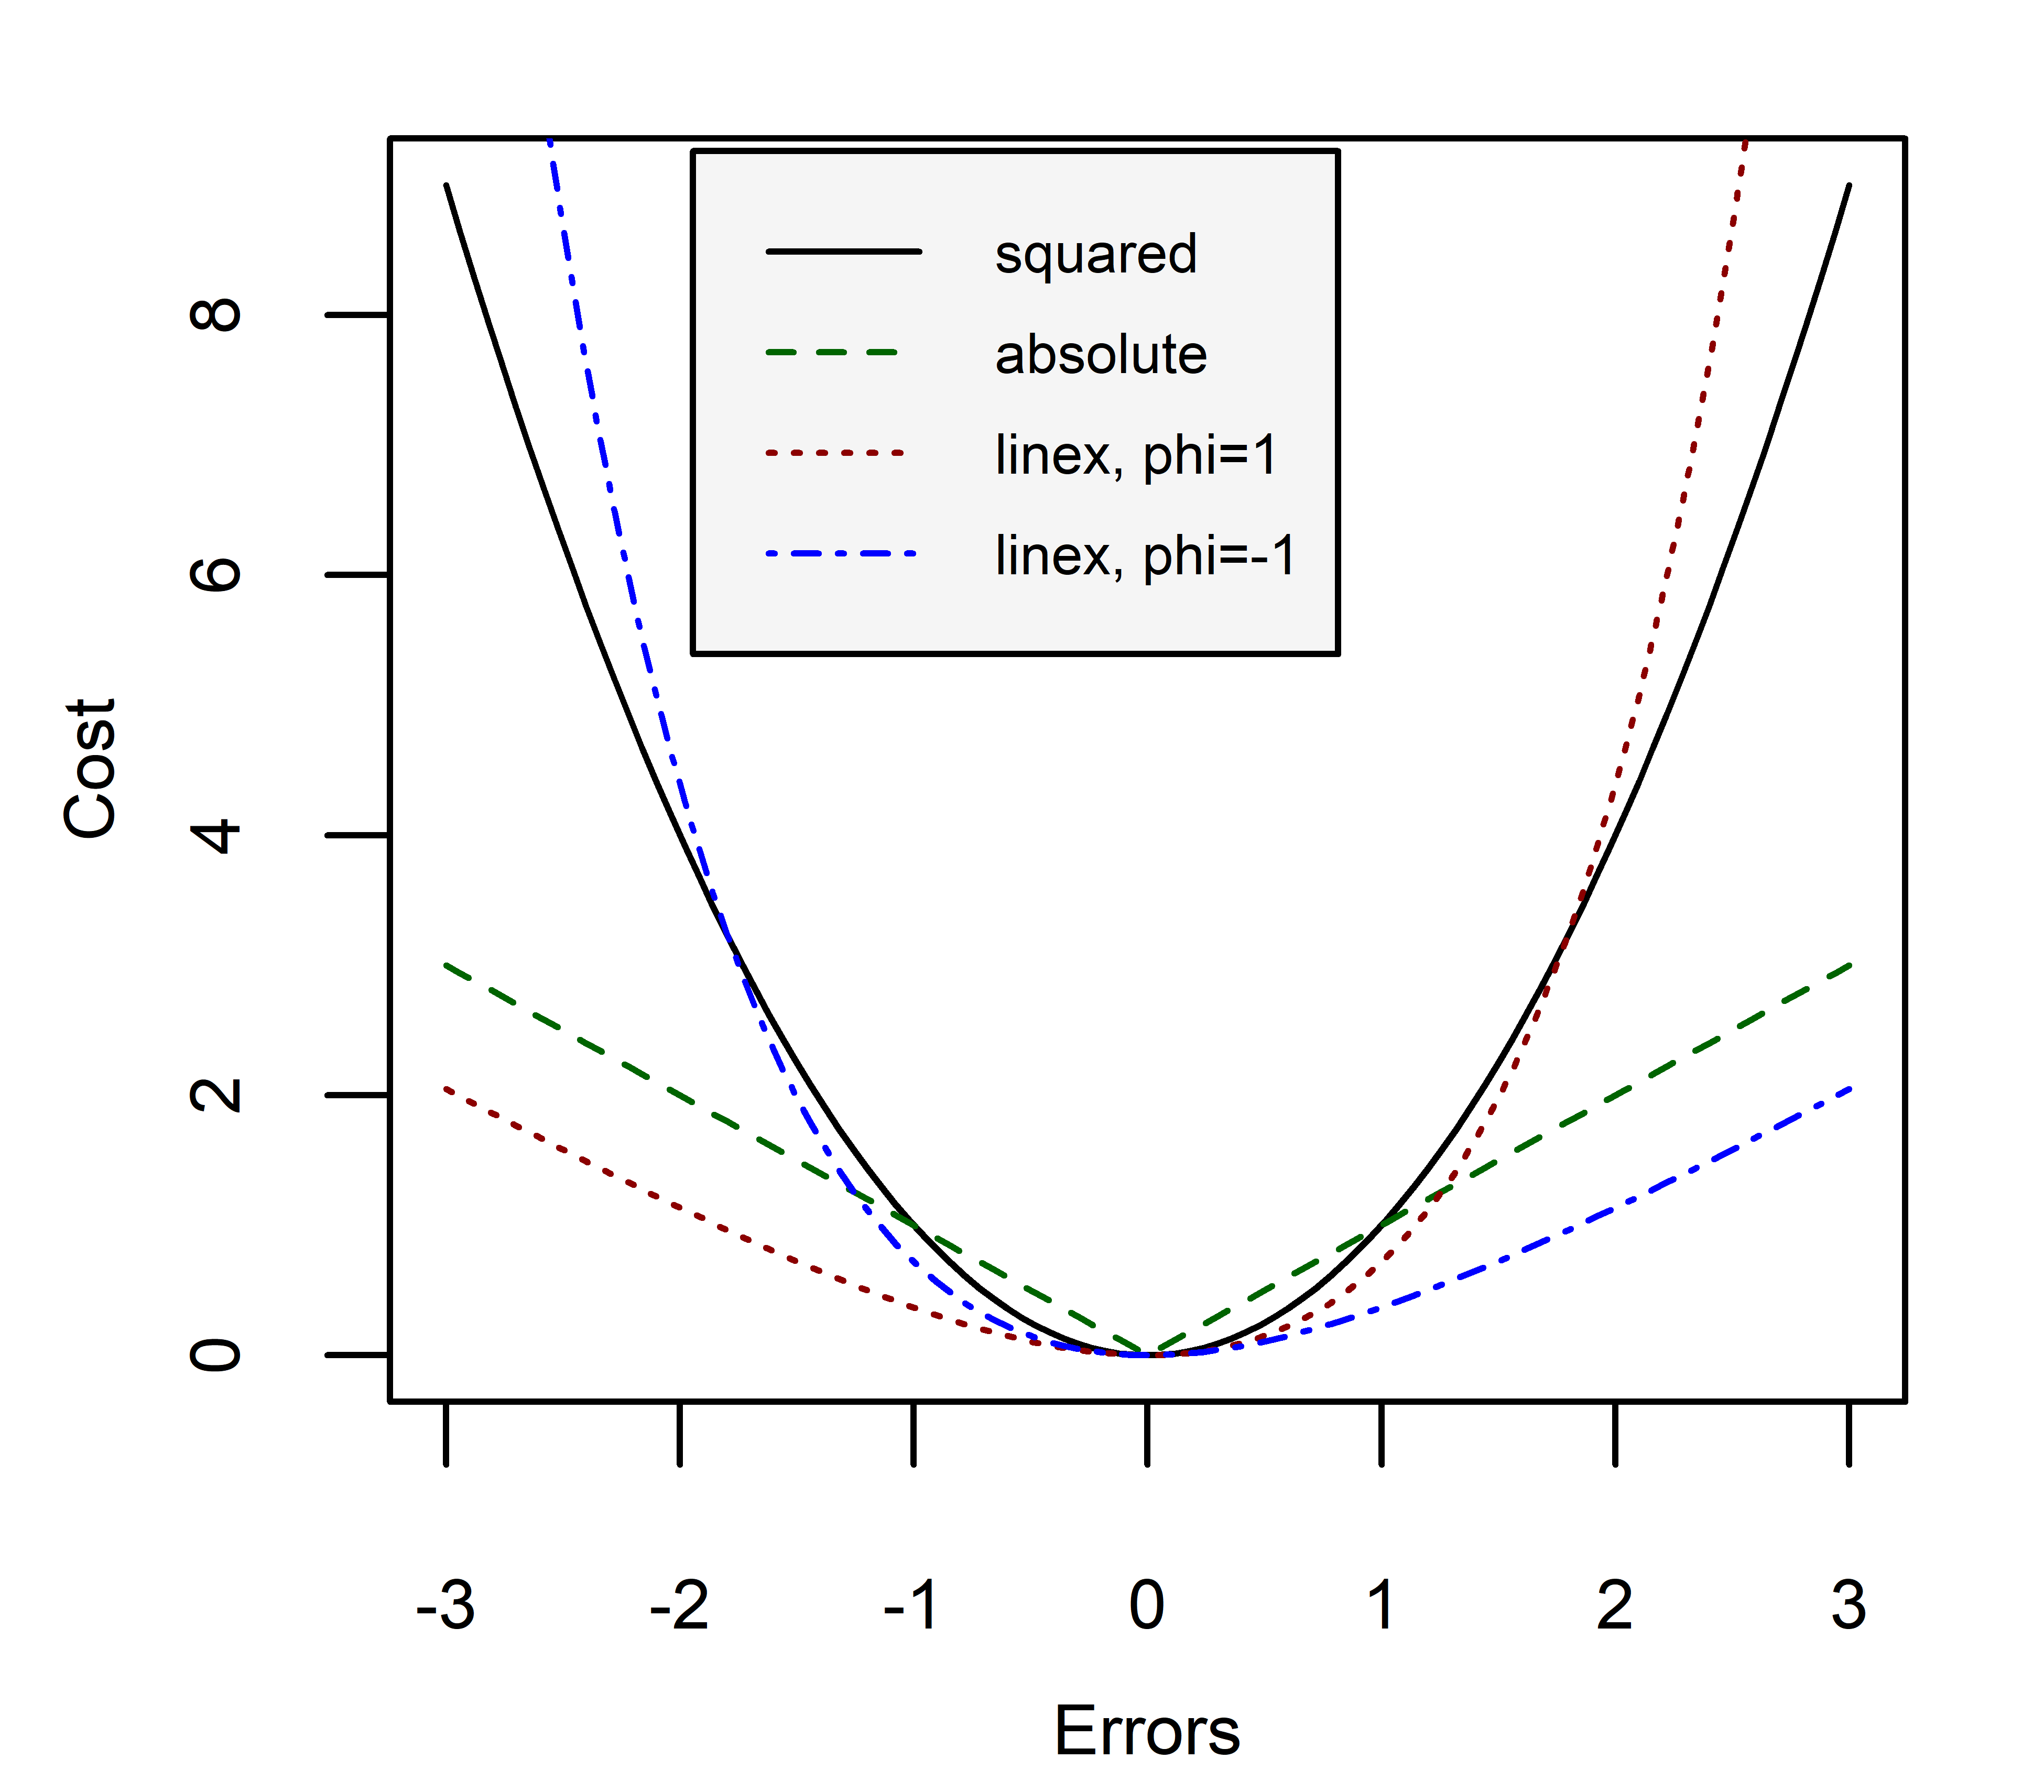
\includegraphics[width=0.7\textwidth, trim={0 0 0 0}, clip=true]{Plots/rplot_lossfuncs.png}
	\caption{Typical loss functions in statistical learning.}
\end{figure}

\textbf{Convex Optimization Problems}: Optimization problems that are convex in the objective function and constraints have a special property; if a solution is found to the minimization or maximization it is guaranteed to be a global solution. 

\textbf{Gradient-Based Optimization Methods}: These methods find the local minima or maxima of an objective function by searching along the gradient of the objective function. For example, in a minimization problem using the steepest gradient search methods, the decent direction and step size is found in one iteration. Gradient-based methods require the loss function to be differentiable. However, variations such as subgradient methods have been developed that allow for the minimization of convex problems given kinks in the loss function. 
 
\textbf{Derivative-Free Optimization Methods}: These methods do not require gradient calculations and are well suited to problems where a loss function is not explicit. For example, evolutionary algorithms find local minima or maxima by evaluating the loss function on a population of solutions, and letting them evolve in each iteration. 

%----------------------------------------------------------------------------------------------------------------------------------------------------------------------------------------------------------
\section*{Learning Scenarios}
\textbf{Supervised vs. Unsupervised}: In supervised settings, we have a variable of interest, $y$, that we believe follows a functional form: $y=f(x)+\epsilon$, where $f(x)$ provides systematic information about $y$, and $\epsilon$ is the error term. In modeling we try to approximate this functional form (i.e., $\hat{f}(x)$) with the observations (i.e., $\hat{y}$). We also can try to estimate y from the data itself, without assuming a functional form (See next section on Parametric vs. Non-Parametric). 

In unsupervised learning, we do not have a variable of interest, $y$, to model. Instead, we have observations of many variables that we can still study for their natural groupings, patterns, or relationships between variables.

\textbf{Prediction vs. Inference}: The two major goals of statistical analysis is either prediction or inference. In prediction, we are interested in getting the simulated value to closely resemble the observed values (e.g., can we accurately predict the value of a house). That is, we are concerned with accuracy. 

However, in inference, we are interested in the relationship of the predictor variables to the response variable (e.g., how much extra will a house be worth given a scenic view). That is, we are concerned with model interpretability, which implies that a simpler (i.e., fewer variables, less flexible) model is preferred even at a little cost to prediction accuracy \cite{james2013introduction}. 

\textbf{Parametric vs. Non-Parametric}: Parametric models assume a functional form. For example, from Ohm's law ($V=IR$), we can safely assume that given an unknown resistor, voltage and current have a linear relationship ($y=\beta_1x+\epsilon$), where y is the voltmeter readings and x is the ammeter readings. By assuming this functional form errors in observations can be due to the measurement device (the voltmeter or ammeter) or human error. Now, we can estimate the parameters of the model from the observations. In this case, we are estimating R, resistance, from fitting $\hat{y}=\hat{\beta}_1x$. We have effectively reduced the problem of finding $\hat{f}(x)$ to finding $\hat{\beta}_1$. 

However, in non-parametric models, we do not assume a functional form and try to get the model as close to the data points as possible without being too ``rough". For example, Kriging interpolators are known to be exact interpolators where the predictions at each observation point goes through the exact observation. Therefore, this approach is highly dependent on the observation and suffers from high variance in the bias-variance trade-off. Smoothing techniques, such as thin plate splines, relax this constraint, and depending on the degrees of freedom or flexibility we allow, the prediction can get close to or far from the observations. This approach is data intense and usually performs better where prediction, rather than inference, is concerned, because, after all, it is more or less honoring the data.

\textbf{Regression vs. Classification}: Variables can be classified as quantitative or qualitative. Quantitative variables take on numerical values and a quantitative response variable is used in what we refer to as regression models. In contrast, qualitative variables take on classes, categories or levels and a categorical response variable is used in classification models. The predictors may take either form and are generally less important \cite{james2013introduction}. 

